\documentclass[a4paper,11pt,english]{article}
\usepackage{amsmath}
\usepackage{gensymb}
\usepackage[english]{babel} 
\usepackage[T1]{fontenc}
\usepackage{lmodern}   
\usepackage[utf8]{inputenc} 
\usepackage{graphicx}       
\usepackage{hyperref}
\usepackage{pgfgantt}
\usepackage{lscape}

\begin{document}

\title{Active strategies for object discovery}
\author{Phil Bradfield \and Jan Fabian Schmid}
	
\maketitle 

\section{Introduction}
Our project is to develop an autonomous mobile system for object detection.
% Instead of using only single images to find positions and shapes of objects in an environment, a mobile system can use a sequence of images from different viewpoints.
It is desirable for an autonomous robot that it is able to interact with and use objects in its environment.
However, in order to do this it has to be aware of the precise locations of objects in order to manipulate or classify them.
For this task object detection can be used.
An object detection algorithm provides a list of object proposals to be analyzed in further detail, meaning that we can focus our object classification systems on promising areas in an image rather than blindly searching.
Such restrictions are necessary, because every mobile system bears certain limitations to its capabilities, particularly regarding processing power, energy and response time.

Usually object detection algorithms only work on single 2D images \cite{atanasov2014nonmyopic}.
A mobile system, however, can produce a sequence of images of a scene during its exploration of the environment.
This produces a number of additional challenges to the traditional 2D problem that we have to deal with.
One is that at each new viewpoint a new set of object proposals is calculated, and these have to be fused with previous object proposals.
The second big problem is that the robot has to decide where to move to next in order to best improve its knowledge of the environment.
This is the problem of finding the next best view (NBV). 
For our project the goal is to analyze and evaluate multiple possible NBV-algorithms in their capability of finding good viewpoints to examine the environment.\medskip

This intermediate report is structured as follows:
The next subsection of this introductory chapter presents the three application scenarios that we want to test our system in.
Then some related work is described.
The presented publications solved similar problems to the ones we encounter.

In Chapter \ref{background} we will go into detail of some of the used approaches in our system.

Following, Chapter \ref{system} will provide an overview of the information flow in our system, and some steps will be described in more detail.
We also describe the current progress and speculate about possible extensions to the system.

Finally, in Chapter \ref{timeline} we will indicate how we will proceed to work on the system and our anticipated timeline. 
 
\subsection{Application scenarios}
Currently three scenarios of application with different complexity are planned.
\begin{itemize}	
	\item \textbf{Table scenario}: Objects of different size, shape and color are assembled on a table.
	Some objects are partially or completely occluded by other objects, therefore a single viewpoint is not sufficient to detect all objects.
	The mobile system has an RGB-D camera mounted at an appropriate height to look on the table.
	It can move freely around the table to reach different viewpoints.
	\item \textbf{Pre-recorded images scenario}: This scenario is only an intermediate application for testing during the development of the system.
	We utilize the same setting as in the table scenario, but without an autonomous system.
	Using an RGB-D camera on a tripod, we take pictures from different viewpoints of the table.
	The system can use these images for object detection and computation of an NBV.
	\item \textbf{Scattered objects scenario}: In this scenario objects lie scattered on the floor.
	The mobile system can move in between the objects to take views on different areas of the scene.
	This scenario is more demanding on the abilities of computing the NBV and moving the robot to the desired viewpoints, which should allow us to examine the pros and cons of different NBV-algorithms.
\end{itemize} 

\subsection{Related work}
In this chapter we introduce some other approaches in which similar problems to those that we address with our system have been solved.\medskip

García and Frintrop build a framework for 3D object detection by utilizing a visual attention system \cite{garcia2013computational}.
They work with a recorded video stream from an RGB-D camera.
The color and depth stream are separately processed. 
The color stream is used to create so called proto-objects, which are areas with high probability of being part of an object.
These proto-objects correspond to the peaks in the calculated saliency map. 
Simultaneously, the image is segmented into areas of pixels with similar color. 
Where proto-objects overlap, they are considered to be a single proto-object and are united to a single object candidate.

At the same time, the depth stream is used to build a map of the scene.
By projecting the object candidates into the 3D map they are able to label voxels as associated to a certain object in the scene.
An inhibition of return (IOR) mechanism for three dimensional scenes is used to allow the algorithm to focus on one salient region after the other.

We can use this framework as a starting point for our project.
As the framework is used for pre-recorded videos, the active sensing part that we need is missing.
Apart from that, we can use the described methods for object candidate creation and the fusion of data from multiple views.
For our project it may not be necessary to implement a 3D IOR map.
This is because we don't have to use a continuously moving video stream to find object candidates.
In our case it is possible to stop movement at our desired viewpoints and take a picture from which object candidates are determined. \medskip

Meger et al. created Curious George, a mobile system that has been successful in the past in object recognition tasks \cite{meger2010curious}.
The robot is given a set of objects, and computes a visual classifier for each in a training phase.
Afterwards the robot drives autonomously through an environment, simultaneously exploring and searching for the known objects.
To build this map and navigate in it they have to solve the Simultaneous Localization and Mapping (SLAM) problem.
This is done with GMapping, which produces a 2D occupancy grid map from laser scan and odometry data (see Section \ref{system:slam}).

Curious George analyzes its environment in two steps.
At first, the robot is guided by a frontier-based exploration algorithm, until a map of the whole scene is built.
Then, as a second phase, the scene is analyzed in more detail.
They use an attention system with a saliency map (comparable to the one in the approach of García and Frintrop) to find interesting places in the already discovered environment.
Saliency is used to focus the attention of the system on relevant parts of the environment.
This is necessary as many possible views are redundant or promise only a very low information gain.
Therefore, visual saliency is used to evaluate the potential information gain of an area; additionally, the environmental structure is analyzed to find areas like desks where a high amount of objects is to be expected.

Even though the system of Meger et al. does object recognition instead of object detection, some parts of the system can be adopted by us.
We have to perform SLAM as well, and Meger et al.'s system shows that GMapping is an applicable solution for this type of problem.
Our robot has no laser range-finder to generate laser scan data, but with the depth data from Kinect we can simulate such data.
The two steps of exploring is also an interesting idea that we can keep in mind for our system.
And as a first approach for a simple NBV-planner we will use a frontier-based exploration algorithm. \medskip

Li et al. presented an online system for incremental scene modeling \cite{li2016incremental}.
They combine the capabilities of a SLAM-based scene understanding framework with semantic segmentation and object pose estimation.
Their goal was to build a multi-view recognition system that works fast and with the necessary accuracy required for robotic application scenarios.
As in our scenario, they take advantage of having a mobile camera to take multiple observations of the same scene, using them to improve recognition abilities.
They train object models on a large set of partial views, and also construct a background model through a provided sequence of scene views without any objects in them.
During application, a set of object hypotheses is updated with every new frame from an RGB-D camera sequence.
To find corresponding spatial areas at the different viewpoints they use the estimated current camera pose from a dense SLAM method.
In their results they reach improved performance in respect to single-view methods for semantic segmentation and object pose estimation.

In our use case the robot doesn't get object models to learn classifiers that can be used during application.
Therefore, this approach is not feasible for us.
However, their work does clearly show the advantage of multi-view object recognition over single-view methods.
The method of fusing multiple views through knowledge of the current camera position seems to be the standard approach, which we can be apply to solve this problem in our system.

\section{Theoretical background}
\label{background}
In this section we will introduce in more detail the methods that we will utilize for our system.

\subsection{Saliency-based object discovery}
\label{background:saliencyobjectdiscovery}
We perform will 2D object discovery on RGB images with a saliency-based approach.
Our method closely follows the approach of García et al. \cite{garcia2015saliency}, which is summarized below.

In their paper they introduce a saliency-based object discovery method using RGB-D data with a late-fusion approach, which means that color and depth object candidates are computed separately and then combined.
This method stands in contrast to early-fusion approaches in which the computation of object candidates is directly performed on the RGB-D data.
An example of such an approach is Voxel Cloud Connectivity Segmentation \cite{papon2013voxel}. 

The method of García et al. consists of four steps:

\begin{enumerate}
	\item First, salient blobs in the image are calculated.
	A salient region is a region in the image with high contrast to the surrounding.
	The contrast of a specific region can be calculated in terms of several different features (e.g. the intensities of different color channels) in parallel.
	To find salient blobs, their first step is to calculate a saliency map with the VOCUS2 system \cite{frintrop2015traditional}, which considers red/green, blue/yellow and intensity center-surround contrasts.
	Then the salient blobs are computed with seeded region growing on the local maxima of the saliency map.
	\item The second step, which happens simultaneously with the salient region extraction, is to segment the image.
	They use four different segmentation methods:
	\begin{itemize}
		\item Felzenszwalb and Huttenlocher's segmentation algorithm \cite{felzenszwalb2004efficient}, which only considers color.
		\item Surface clustering searches for surface patches in the depth data.
		\item The previously mentioned Voxel Cloud Connectivity Segmentation for an early-fusion approach.
		\item And the late-fusion approach of separately computing candidates from color and surface segments and then combining them.
	\end{itemize}	   
	\item For candidate generation the information of salient regions and segments is brought together.
	An object candidate consists of multiple segments, which results in precise boundaries of the candidates.
	For each salient region the set of overlapping segments is selected as an object candidate.
	\item The last step is to rank the computed candidates.
	They compare three different ranking methods:
	\begin{itemize}
		\item A score calculated as average saliency multiplied by the square of the area of the candidate.
		\item 3D convexity.
		\item A range of features that are learned by a SVM.
	\end{itemize}
\end{enumerate}

They conclude from the comparison of the different methods that the late-fusion approach performs best.
Using the SVM for candidate ranking has a much higher precision when only considering a few object candidates; however, the performance of the three different approaches is more similar for recall and it converges with a higher number of object candidates.

\subsection{Sampling-based exploration}
\label{background:surmann}
Surmann et al. developed a system for autonomous digitalization of 3D indoor environments \cite{surmann2003autonomous}.
This system consists of three core modules: a mapping algorithm, a view planner and a navigator to move the robot to a desired goal.
Especially interesting for us is how they compute a NBV.
A view planner is necessary in this scenario because many possible views promise only a very low information gain and the amount of views that can be used is limited by time and energy constraints.
A visualization of the steps of their method to find the NBV can be seen in Figure \ref{fig:surmann}.

\begin{figure}[h!]
	\begin{center}
		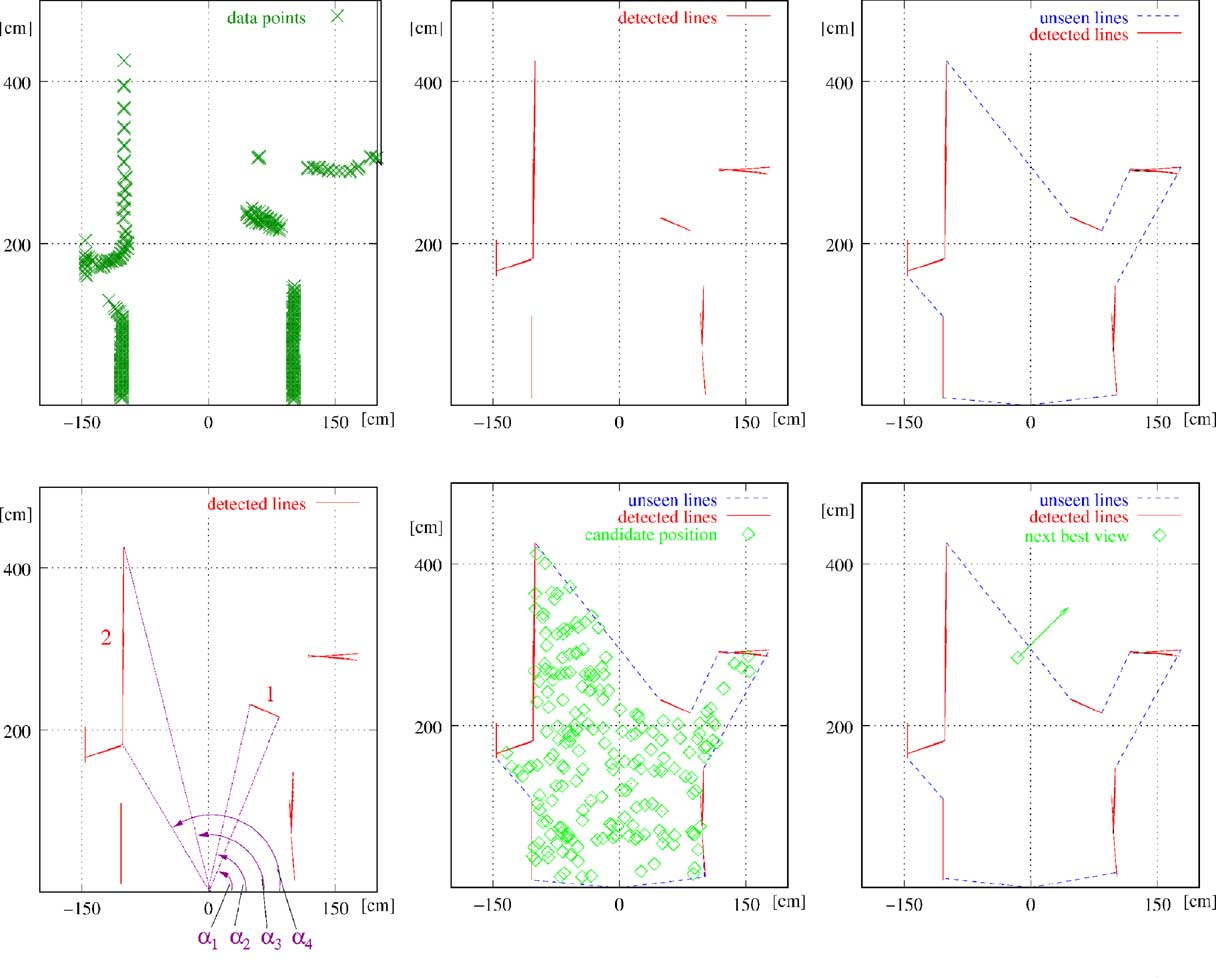
\includegraphics[width=1\textwidth]{src/nbv.png}
		\caption{Next best view planning as it is done in the approach of Surmann et al. \cite{surmann2003autonomous}}
		\label{fig:surmann}
	\end{center}
\end{figure}

To compute the next best view they generate multiple horizontal 2D layers of their 3D map of the environment.
An example of one of these layers is pictured in the first frame in Figure \ref{fig:surmann}.
The green crosses represent single data points from the laser range finder.

They use Hough transform to find lines in the layer which represent the obstacles (e.g. walls) they already detected (frame 2).

The lines are then connected by ``assumed lines'' to form an estimate of the layout of the room (frame 3).

In frame 4 it is shown how the assumed lines are calculated, using the example of the assumed line between the actual lines numbered 1 and 2. 
The endpoints of the actual lines are sorted by their increasing polar angle counterclockwise.
Actual lines with neighboring endpoints in that sorting are then connected by assumed lines.

The next step is to randomly generate possible viewpoints in the already discovered space, which are pictured as green squares in frame 5.
For each viewpoint $p$ the information gain $V(p)$ is calculated as a measure of how many assumed lines can be seen from it.
A compromise between traveling distance and information gain is then used to decide on the next viewpoint.
The score $S(p)$ for the viewpoint $p$ is calculated as $S(p) = V(p) exp(-c_1||r-p||)exp(-c_2||\Theta_r-\Theta_p||)$, where $r$ is the position of the robot and $\Theta_r$ its current orientation, $p$ the position of the viewpoint and $\Theta_p$ the orientation of the viewpoint. The terms can be weighted with the constants $c_1$ and $c_2$.

The NBV is chosen as the sample with highest score.

\section{System description and progress}
\label{system}
A general overview of our system is given in Figure \ref{fig:overview}.

\begin{figure}
	\begin{center}
		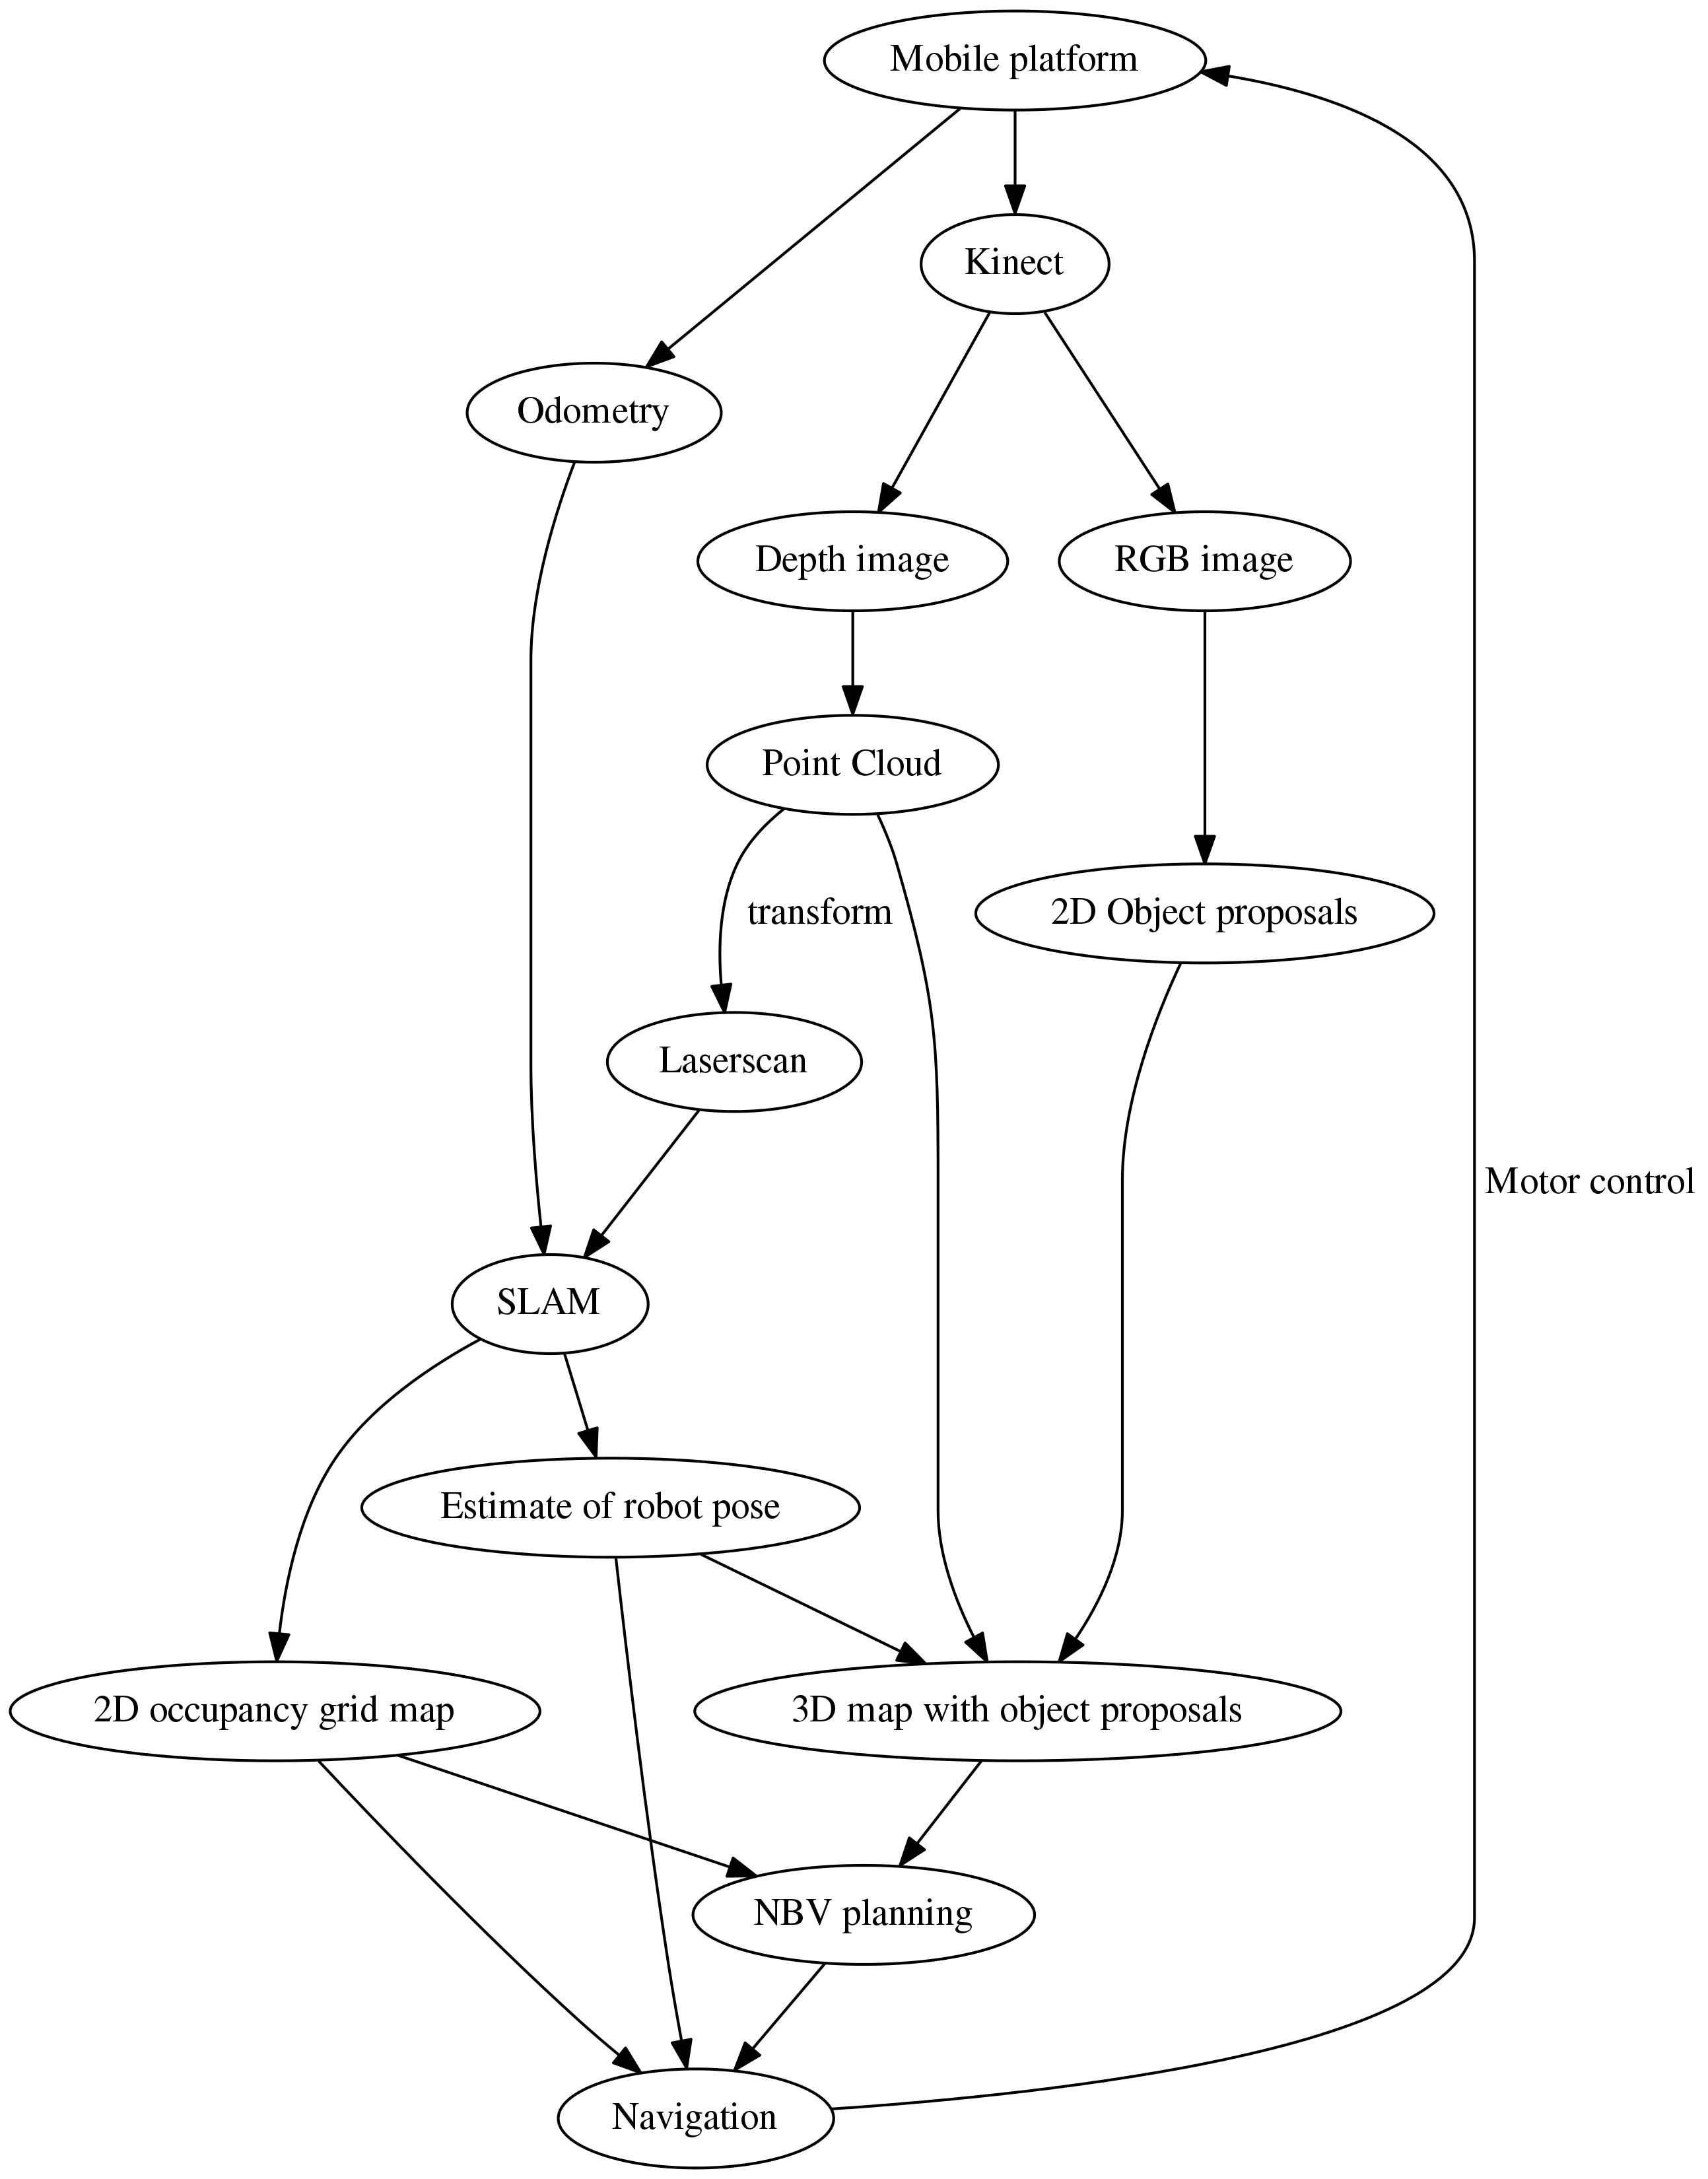
\includegraphics[width=1\linewidth]{dot/overview.png} 
		\caption{Overview of the system}
		\label{fig:overview}
	\end{center}
\end{figure}

Before we start explaining the graph in detail, it is useful to have a look at the available input and the desired output of our system.
\begin{itemize}
	\item \textbf{Input:}
	\begin{itemize}
		\item We will use a mobile platform like a Pioneer or Turtlebot, which provides odometry data from the motion sensors.
		\item Onto the mobile platform we mount a Kinect camera, which provides RGB-D images of the scene.
	\end{itemize}
	\item \textbf{Output:}
	\begin{itemize}
		\item During operation of the system it is moving around the scene.
		Therefore, motor control can be seen as intermediate output of the system.
		\item The goal is to retrieve a 3D map with incorporated labels of all found object proposals.
	\end{itemize}  
\end{itemize}

Independent of the used application scenario the robot starts with no pre-knowledge of the scene.
Therefore, we are completely dependent on the system input to infer information.

At the beginning only an initial RGB-D image of the robot viewpoint at the start is available.
One processing line uses the RGB image to find any possible objects in the view; this is described in detail in Section \ref{system:obj_discovery}.

Simultaneously the depth image of the Kinect camera is processed.
From the depth data a point cloud is computed; this is used to simulate laser-scan data, which consists of depth data of one horizontal line in the robot view. 
This laser scan data is used together with the odometry data to perform simultaneous localization and mapping.
This part is described in more detail in Section \ref{system:slam}.

The SLAM algorithm provides a 2D occupancy grid map, which is a kind of floor plan containing information about obstacles and free space in the already discovered environment.
A second output of SLAM is an estimate of the current robot pose.
This pose is used together with the newly found object proposals from the current view and the current depth image to update the 3D map that contains a labeling of voxels to object proposals.
This procedure is specified in Section \ref{system:fusion}. 

The next step is to compute an NBV for the robot that should maximize the information gain about the environment.
For this computation all data that has been gathered to this point can be used; in particular the positions of previously found object proposals and the current floor map will be used for this step.
Details can be found in Section \ref{system:nbv}.

Once a desired view point is calculated, it is used together with the current occupancy grid map and pose estimation to plan movement of the robot to this point in space.
This part is described in Section \ref{system:navigation}.

The output of the navigation module is the motor commands to move the system.
During movement the SLAM algorithm is constantly processing the camera data to update the map and keep track of the robot position.
Once the viewpoint is reached another image of the scene is taken, and the next iteration of the object detection process starts.

After describing the individual parts of our system in more detail, the last subsection of this chapter provides a short list of possible extensions to the system, that we will work on if time permits.

\subsection{Object discovery in two dimensions}
\label{system:obj_discovery}
To find object candidates, we use a part of the method from García et al. described in Section \ref{background:saliencyobjectdiscovery}.
For simplicity, we will only use color candidates; the use of depth candidates that are then fused with the color candidates is a possible extension for our project.
Our object discovery works as follows: First we calculate a saliency map with VOCUS2 \cite{frintrop2015traditional}, then we iterate over local maxima in the map to calculate salient blobs with seeded region growing.
That means that all pixels neighboring the currently considered local maximum are taken as part of the salient region if their saliency value is at least \(x\)\% or more of the saliency value of the maximum.
This process is done once with 60\% and once with 70\% similarity requirement.
A salient region is only kept if it has at least a mean saliency value of 120 (from a maximum of 255) in order to only keep actually interesting regions.
Some of the salient regions will overlap each other, if the overlap is greater than 50\% only the one with higher saliency score is kept.
The saliency score is calculated as mean saliency times square root of the area of the corresponding region.
The segmentation is done using a C++ implementation of the Felzenszwalb and Huttenlocher algorithm \cite{felzenszwalb2004efficient} by Christoffer Holmstedt \footnote{\url{https://github.com/christofferholmstedt/opencv-wrapper-egbis}}.
For each remaining salient region an object candidate is now calculated by finding all segments that overlap with at least 30\% with the region.

This part of our system is already implemented as a C++ class and is working.
To use it with the mobile platform, we will have to write a wrapper for ROS for it.

\subsection{SLAM}
\label{system:slam}
To perform simultaneous localization and mapping we use a ROS wrapper\footnote{\url{http://wiki.ros.org/gmapping}} for OpenSlam's GMapping algorithm \cite{grisetti2007}, which is an implementation of Fast SLAM.
It uses laser scan and odometry data to compute a 2D occupancy grid map of the discovered environment.
The algorithm requires laser scan data from a horizontally-mounted laser range-finder.
We don't have such a laser range-finder; however, we can transform the depth image provided by the Kinect camera to laser scan data.
Therefore we have to define the height for which the horizontal laser range data is computed.
Because the data is used for navigation the height should be at ground level.

The ROS wrapper provides topics to retrieve the built 2D occupancy map and the current pose estimation of the robot in this map.

\subsection{Object discovery in three dimensions}
\label{system:fusion}
Once object proposals have been generated from the RGB image using the saliency system, the pixel-based object proposals will be translated into 3D voxel-based proposals.
This will by done by using the Kinect's depth map to project the 2D object proposals into a 3D space; each voxel in the 3D space which corresponds to part of a proposed object surface will be assigned the label of that proposed object, and a score representing the confidence with which we are labeling that voxel with each different label (i.e. a single voxel can have multiple labels, each with their own confidence score).

For each new viewpoint that the robot reaches, new 2D object proposals will be generated and these will be used to update the existing voxel labels.
First, the 2D object proposals will be projected into the existing 3D space.
The robot pose estimate from the SLAM system will give us the initial point and direction from which to perform the projection; combining this information with the depth map from the Kinect will give us the full transformation into the 3D space, telling us which voxels each new proposal occupies.
We will then use the newly generated proposals to update the existing ones, taking our basic strategy from \cite{garcia2013computational}:

\begin{itemize}
	\item If less than 5\% of the voxels in the new proposal are already labeled, then the voxels in the new proposal will be assigned to a new label and confidence score, as before.
	\item Otherwise, we will search over the voxels in the new proposal and find the existing label \(l\) which occurs most often (i.e. the existing proposal which most significantly overlaps the new one).
	Any voxels in the new proposal which are not labeled as \(l\) will be assigned label \(l\) with an initial confidence level.
	For each voxel in the new proposal, all labels which are not \(l\) will have their confidence levels decreased.
	If a label's confidence score falls below a threshold then it is deleted.
\end{itemize}

The initial confidence score of a newly-added label will be low, as the idea of the fusion process is that proposals which truly correspond to objects will be repeated often and thus build up confidence quickly, while false proposals which are not replicated should be quickly flushed from the system in order to keep the computation manageable.
The exact initial value of the confidence score, and the magnitude of the increase or decrease in confidence at each update, will need to be empirically determined.

\subsection{Determining the next best view}
\label{system:nbv}
After processing the image data from one viewpoint the robot has to decide where to go next.
This step is the core of our system and our main research focus.
The goal is to find object candidates with a high level of both precision and recall, i.e. we create the minimum possible number of candidates which do not match to objects in the scene, and we create closely matching candidates for all objects actually present in the scene.
The computation of the NBV determines the strategy how to reach this goal.

Desirable properties of the NBV algorithm are:
\begin{itemize}
	\item The computed NBVs should maximize the information gain on the scene.
	It is not necessary to process images from the same or similar viewpoints multiple times.
	Also the view should focus on regions containing objects and on regions with high uncertainty about the object candidates.
	If the remaining energy of the robot has a value associated with it, at some point the predicted information gain has less value then the required energy to reach the NBV.
	At this point our system can terminate.
	\item The computational cost should be reasonable.
	Because of the constraints of energy and time in mobile systems, the value of a very good NBV against a mediocre NBV has to be considered against the additional effort required to compute the better NBV.
	It is probably not appropriate if the energy or time consumption for calculating a very good NBV and moving to it is as high as calculating and moving to two mediocre NBVs.
	This is especially important in our use case, because exploring the whole scene is already a very important aspect of a good next viewpoint.
\end{itemize}

We want to implement and evaluate multiple NBV algorithms during our project.
We will then evaluate their ability to find objects in the scene and how long and how much energy each one took.

In the following subsections we will explain in detail the different NBV algorithms that we plan to implement.

\subsubsection{Frontier-based exploration}
This approach is very simple, without much computation going into the NBV.
The goal of this method is to find viewpoints that are suitable in order to explore the whole scene, which is something an autonomous robot has to do in a new environment anyhow.
No further effort is taken to focus on objects in the environment, objects are discovered as a side-product of the exploration process.
The performance of this simple approach will be used as baseline to evaluate the gain of more sophisticated approaches.

In frontier-based exploration the robot is always moving to the nearest reachable frontier.
A frontier is defined as a border region between explored free space and unexplored space, and a frontier is reachable if a path from the current robot position through the known free space to the frontier position exists.

Frontier-based exploration has been implemented in a ROS-package \footnote{\url{http://wiki.ros.org/frontier_exploration}} that we plan to use.

\subsubsection{Information gain approach}
This NBV method is based on the approach described in Section \ref{background:surmann}.
We plan to implement two variations of this approach: one directly using Surmann et al.'s method of calculating information gain based on the number of assumed lines a potential next viewpoint can see; another which calculates information gain based on attempting to reduce the uncertainty in our labeling.
A combination of the two approaches will also be attempted.

\paragraph{Unseen lines}
The basic intention of Surmann et al.'s approach is to explore an indoor environment.
In applying the approach to NBV, our system will sample the already discovered environment and find the viewpoints which allow a view on as many assumed lines as possible.
The system will then calculate a trade-off between the potential information gain offered by a potential next viewpoint and the amount of time it would take the robot to get there.
Exploration is an important aspect that has to be considered by our NBV planner, because the robot can only find all objects when it has at least looked in all general areas of the room once.
In our system an occupancy grid map is computed at ground level for navigation purposes; to use the Surmann et al. approach, we compute another 2D grid map for the height at which the objects are located.
The whole method is then performed on this 2D grid map.

\paragraph{Label uncertainty}
For the purposes of NBV calculation, an alternative formulation of information gain would be to look at the uncertainty of the labels in our voxel map.
Areas of the map which have high uncertainty would be areas which have either not been viewed at all (which would have maximum uncertainty) or areas in which our system has previously generated contradictory labels, denoting an area which needs further investigation.
As with the assumed lines approach, the system would calculate the information gain for each sampled viewpoint, and then select the next viewpoint by means of a trade-off between the viewpoint's potential information gain and its distance from the robot's current location.

\paragraph{Combination}
The two approaches above could also be complementary, with information gain being calculated using the sum of both measures, possibly with a weighting factor.

% \paragraph{}Further adaptations to the information gain measure could also be possible, such as extending the unseen lines approach by extrapolating from the already found object surfaces.
% Rather than simply positing straight lines between points, the system could use heuristics to generate the unseen lines, for example assuming that a flat surface which vanishes into unseen space continues to be a flat surface in that unseen space.
% Similarly, a partially-seen surface with constant curvature could be assumed to continue to have the same curvature in in its unseen sections.
% This idea is tangentially related to Gestalt principles

\paragraph{}
This part is not implemented yet.

\subsection{Navigation}
\label{system:navigation}
Navigation will be handled using the ROS Navigation Stack\footnote{\url{http://wiki.ros.org/navigation}}.
Once the next best view processor has decided where the robot should next observe the scene from, this target pose will be sent to the navigation stack along with the applicable co-ordinate frame transformations.
The navigation stack will then plan a path to the target position and formulate the motor commands to move the robot along the path.

In the table scenario, successfully moving the robot to the target position should be relatively straightforward because we will be able to keep the robot's area of navigation clear, meaning there are no obstacles for the robot to avoid.
The scattered objects scenario represents a greater challenge to the navigation system as the objects which the system is trying to detect also automatically become obstacles that it has to avoid, and thus the robot's path planning becomes more complex.
Additionally, in the scattered objects scenario the robot may potentially have to search for objects in a full 360\degree\ radius around its starting position, whereas in the table scenario the robot only needs to focus on a single area of interest.

This part of the system is not implemented yet. It is expected that the effort required to implement this is low, as we are simply using existing ROS functionality and do not need to customize the navigation system ourselves in any way.

\subsection{Extensions}
\label{system:extensions}
In the following list we present possible extensions to the core system that has been described so far. 
The extensions could improve the system and may be implemented if time permits, but they are not essential for its abilities.

\begin{itemize}
	\item Depth information for the computation of object proposals.
	As described in Section \ref{system:obj_discovery} we only use color candidates, but in the work of García et al. we summarized in Section \ref{background:saliencyobjectdiscovery} they showed that the additional usage of depth information which is integrated in a late-fusion approach can significantly improve the accuracy of saliency-based object discovery.
	\item An extension to the assumed lines approach which uses heuristics to improve on the estimation of unseen surfaces, e.g. by assuming that a flat surface which disappears into unknown space continues to be flat and that a curved surface continues with the same curvature.
	\item An additional NBV planning algorithm that exploits POMDPs.
\end{itemize}

\section{Timeline}
\label{timeline}

The Gantt chart in figure \ref{fig:timeline} presents our time plan for the project.
The chart contains the different tasks we still have to work on and a rough time schedule for them.
The two black diamonds represent significant milestones for the project.

Our timeline starts on 27\textsuperscript{th} March; this start date reflects the fact that the project is likely to be largely dormant during March due to other commitments.
As the final deadline for the project is not concretely fixed, we have chosen to work towards what we judge to be the earliest likely deadline: 16\textsuperscript{th} July, the final day of the teaching period of summer semester 2017.
Planning to be finished by this date will allow us some contingency time, should the final agreed deadline be later than this.

\paragraph{Simulation environment}
In addition to implementing the system as described in section \ref{system}, for the purposes of increasing the speed of testing we will also be setting up a simulation environment using Gazebo\footnote{\url{http://gazebosim.org/}}.
Gazebo already contains modules for simulating small mobile platforms like we shall be using and also the input from a Kinect camera; we shall create application scenarios in Gazebo using the available models of the objects in our dataset.
An advantage of using ROS for our system is that aside from the work of actually creating the application scenarios in Gazebo, there is very little overhead involved in creating this simulation environment.
Any code, launch files etc. which we create which work in the simulation should not need any major structural changes to work on the real robot, although obviously the extra noise and uncertainty present in real world environments means significant real world testing will still be required.
We plan to perform some brief confidence testing on the real world system in mid to late May, while the full transition from simulation to real world testing is scheduled for late June (see below).

The work of creating this simulation environment is currently in progress.

Planned completion date: week ending 23\textsuperscript{rd} April.

% For the purposes of testing we decided that it would be best to set up a simulation environment.
% With Gazebo \footnote{\url{http://gazebosim.org/}} an easy to use simulation environment is available which already contains modules for mobile platforms and the Kinect camera.
% Additionally we will need models of the objects we want to use, which should be available.
% We will build our application scenarios inside the simulation.
% We plan to work in the simulation only until the last weeks in the summer semester.
% Because of knowledge about the exact positions of the objects in the simulation evaluation of the system will be simpler.

\paragraph{Navigation and map building}
Once the simulation environment is created, we will implement the abilities of building a 2D occupancy grid map and navigating through the space.
At this point we reach our first milestone, which is to have a working simulation environment in which the robot can freely roam around and explore.

Planned completion date: week ending 7\textsuperscript{th} May.

\paragraph{Object discovery}
The next step is to create a wrapper to integrate our existing saliency-based object detection system into ROS.
The wrapper should subscribe to a topic at which RGB images are provided and then publish a topic which provides the 2D object candidates.
Alongside this we can implement the fusion of multiple views which maps the 2D object proposals into a 3D data structure that is then updated from viewpoint to viewpoint.
We plan to work on these two modules concurrently as changes in either one may well affect the messaging required between them.

Planned completion date: week ending 21\textsuperscript{st} May.

\paragraph{Frontier-based next best view planning}
With the object discovery system in place, we can implement frontier-based exploration as a baseline NBV planning approach.
This marks our second milestone, which is to have a fully functional system using our baseline NBV planner.
At this point, we may perform some brief confidence testing on the real robot system in order to make sure that there are no large, unexpected differences between the simulation environment and the real world which we need to be aware of in implementing our planners.

Planned completion date: week ending 28\textsuperscript{th} May.

\pagebreak
\paragraph{Information gain-based next best view planning}
The final implementation stage is to implement our information gain-based planners.
As it is likely that one of the planners will be ready before the other, this phase will in reality probably overlap with the following testing and evaluation phases, as one of us can be testing one NBV planner while the other person is still developing the second planner.

Planned completion date: week ending 18\textsuperscript{th} June.

\paragraph{Testing}
In this phase, we will test our system on the real robot platform and make any adjustments necessary to successfully make the transition from simulation to real world operation, such as exploring different possible parameterizations.

Planned completion date: week ending 25\textsuperscript{th} June.

\paragraph{Evaluation}
Finally, we shall perform comparative evaluations in the real world, measuring the performance of the different NBV planners, and prepare the results for presentation.

Planned completion date: week ending 16\textsuperscript{th} July.

\begin{landscape}
% \begin{figure}[htbp]
% 	\begin{ganttchart}[x unit=10mm]{13}{28}
% 		\gantttitle{Calender week 2017}{16} \\
% 		\gantttitlelist{13,...,28}{1} \\
% 		\ganttbar{Simulation environment setup}{13}{16} \\
% 		\ganttlinkedbar{Navigation and 2D map building}{17}{18} \\
% 		\ganttmilestone{Running simulated robot}{18} \ganttnewline
% 		\ganttbar{Object detection - ROS wrapper}{19}{20} \\
% 		\ganttbar{Fusion of views into a 3D map}{19}{20} \\
% 		\ganttlinkedbar{Simple NBV planning}{21}{21} \\
% 		\ganttmilestone{Prototype of system is working}{21} \ganttnewline
% 		\ganttbar{Sophisticated NBV planning}{22}{24} \\
% 		\ganttlinkedbar{Real world testing}{25}{25} \\
% 		\ganttlinkedbar{Evaluation}{26}{27} \\
% 		\ganttlinkedbar{Final presentation}{28}{28} \\
% 	\end{ganttchart}
% 	\caption{Planned timeline of the remainder of the project}
% 	\label{fig:timeline}
% \end{figure}

% \newpage
\begin{figure}[htbp]
	\begin{ganttchart}[
		title label font=\tiny,
		x unit=1.5mm,
		time slot format=isodate,
		vgrid={*6{white},{gray,dashed}},
		hgrid={gray,dashed}
		]{2017-03-27}{2017-07-16}
		% \gantttitle{Date} \\
		% \gantttitlelist{13,...,28}{1} \\
		\gantttitlecalendar{month=name, week=13} \\
		% \gantttitlelist{13,...,28}{1} \\
		\ganttbar{Simulation setup}{2017-03-27}{2017-04-23} \\
		\ganttlinkedbar{Navigation, map building}{2017-04-24}{2017-05-07} \\
		\ganttmilestone{Running simulated robot}{2017-05-07} \ganttnewline
		\ganttbar{Object detection - ROS wrapper}{2017-05-08}{2017-05-21} \\
		\ganttbar{Proposal fusion into 3D map}{2017-05-08}{2017-05-21} \\
		\ganttlinkedbar{Simple NBV planning}{2017-05-22}{2017-05-28} \\
		\ganttmilestone{Prototype working}{2017-05-28} \ganttnewline
		\ganttbar{Sophisticated NBV planning}{2017-05-29}{2017-06-18} \\
		\ganttlinkedbar{Real world testing}{2017-06-19}{2017-06-25} \\
		\ganttlinkedbar{Evaluation}{2017-06-26}{2017-07-09} \\
		\ganttlinkedbar{Final presentation}{2017-07-10}{2017-07-16} \\
	\end{ganttchart}
	\caption{Planned timeline of the remainder of the project}
	\label{fig:timeline}
\end{figure}
\end{landscape}

\newpage
\bibliographystyle{plain}
\addcontentsline{toc}{section}{Bibliography}% Add to the TOC
\bibliography{bib}

\end{document}
